% =====================================================================
% chapters/04-results.tex
% PT: Capítulo 4 -- Resultados. Exemplo de: tabela com booktabs e colunas
%     numéricas alinhadas (siunitx), figura a partir de um ficheiro em
%     figures/, e números no formato português (vírgula decimal).
% EN: Chapter 4 -- Results. Shows: a table with booktabs and aligned
%     numeric columns (siunitx), a figure from a file in figures/, and
%     numbers in Portuguese format (decimal comma).
% =====================================================================
\chapter{Results}
\label{chap:results}

% PT: Parágrafo de abertura do capítulo.
% EN: Chapter opening paragraph.
This chapter shows how to present results in a table and in a figure. In a
real dissertation, the results chapter reports what was measured, in the
order of the research questions, and leaves the interpretation for the
discussion. All values in this chapter are illustrative.

% ---------------------------------------------------------------------
% PT: Exemplo em inglês
% EN: English example
% ---------------------------------------------------------------------
\section{English example}
\label{sec:results:en}

\subsection{Results Table}
\label{sec:results:table}

% PT: Tabela com booktabs: use só \toprule, \midrule e \bottomrule, sem
%     linhas verticais. A legenda das tabelas vai por cima.
%     Colunas S (siunitx) alinham os números pela vírgula/ponto decimal;
%     table-format=2.1 significa 2 algarismos inteiros e 1 decimal.
%     Cabeçalhos de colunas S vão entre chavetas { }.
% EN: Table with booktabs: use only \toprule, \midrule and \bottomrule,
%     with no vertical lines. Table captions go above the table.
%     S columns (siunitx) align numbers on the decimal marker;
%     table-format=2.1 means 2 integer digits and 1 decimal.
%     Headers of S columns go inside braces { }.
\begin{table}[htbp]
  \centering
  \caption{Example of a results table with booktabs and siunitx
    (illustrative values).}
  \label{tab:results}
  \begin{tabular}{l S[table-format=2.1] S[table-format=1.3] S[table-format=2.1]}
    \toprule
    {Method} & {Accuracy (\%)} & {F1-score} & {Training time (min)} \\
    \midrule
    Baseline          & 78.4 & 0.762 & 12.5 \\
    Method A          & 84.1 & 0.829 & 18.0 \\
    Method B          & 86.7 & 0.851 & 25.3 \\
    Proposed method   & 89.2 & 0.884 & 21.7 \\
    \bottomrule
  \end{tabular}
\end{table}

% PT: Números e unidades no texto: \num, \qty e \percent.
% EN: Numbers and units in the text: \num, \qty and \percent.
\Cref{tab:results} compares the proposed method with a baseline and two
alternatives. The proposed method reaches an accuracy of \qty{89.2}{\percent}
and an F1-score of \num{0.884}, while taking \qty{21.7}{\minute} to train.
Bold or colour can highlight the best value, but the table should be
readable without them.

\subsection{Results Figure}
\label{sec:results:figure}

% PT: Figura a partir de um ficheiro. Prefira PDF (vetorial) para gráficos
%     e PNG/JPG para fotografias. A legenda das figuras vai por baixo.
% EN: Figure from a file. Prefer PDF (vector) for charts and PNG/JPG for
%     photographs. Figure captions go below the figure.
\begin{figure}[htbp]
  \centering
  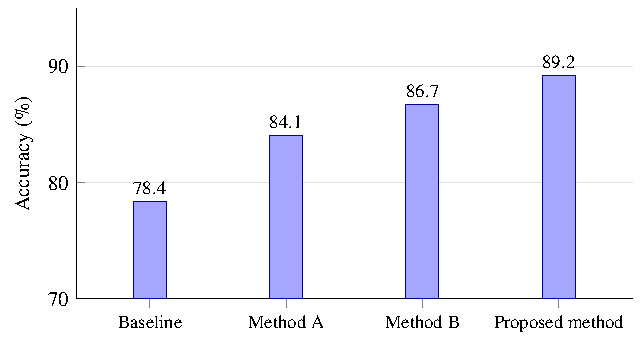
\includegraphics[width=0.75\textwidth]{figures/example-figure.pdf}
  \caption{Example of a figure included from a PDF file: accuracy of each
    method in \cref{tab:results} (illustrative values).}
  \label{fig:example-file}
\end{figure}

\Cref{fig:example-file} shows the same accuracy values as a chart. Charts
are easier to compare at a glance, while tables give the exact values; use
the one that best supports the point you are making.

% ---------------------------------------------------------------------
% PT: Exemplo em português
% EN: Portuguese example
% ---------------------------------------------------------------------
\section{Exemplo em português}
\label{sec:results:pt}

\begin{otherlanguage}{portuguese}
% PT: Formato português dos números só dentro deste bloco: vírgula decimal
%     e espaço fino a separar os milhares.
% EN: Portuguese number format only inside this block: decimal comma and a
%     thin space as thousands separator.
\sisetup{output-decimal-marker={,}, group-separator={\,}}

A Tabela~\ref{tab:results} e a Figura~\ref{fig:example-file} apresentam os
resultados. O método proposto atinge uma exatidão de
\qty{89.2}{\percent} e um F1-score de \num{0.884}, com um tempo de treino de
\qty{21.7}{\minute}, num conjunto de \num{50000} imagens. No ficheiro
\texttt{.tex}, os números escrevem-se sempre com ponto decimal; o siunitx
encarrega-se de os mostrar com vírgula.

\end{otherlanguage}
